\documentclass[a4paper, 12pt]{article}

\usepackage{mathtext}
\usepackage[T2A]{fontenc}
\usepackage[utf8]{inputenc}
\usepackage[russian]{babel}

\usepackage{amsmath}
\usepackage{titlesec}
\usepackage{scrextend}
\usepackage{graphicx}
\usepackage{tikz}

\DeclareSymbolFont{T2Aletters}{T2A}{cmr}{m}{it}
\graphicspath{ {./images/} }

% Установки для отрисовки решеток кодера
\tikzstyle{lightedge}=[dashed]
\tikzstyle{mainedge}=[solid]
\tikzstyle{inputBit}=[rectangle,fill=red, text=white]
\tikzstyle{outputBit}=[rectangle,fill=blue, text=white]
\tikzstyle{pointer}=[orange,->,dashed]

\newcounter{ctra}
\newcommand{\trellisEdges}[2]{%
  \setcounter{ctra}{#2}
  \pgfmathtruncatemacro{\xplusone}{#1 + 1}
  \ifodd\value{ctra}
      \draw[mainedge] (s#1#2) -- (s\xplusone2);
  \else
      \draw[mainedge] (s#1#2) -- (s\xplusone0);
  \fi%
  \ifodd\value{ctra}
      \draw[lightedge] (s#1#2) -- (s\xplusone3);
  \else
      \draw[lightedge] (s#1#2) -- (s\xplusone1);
  \fi%
}

% #1=x; #2=y; #3=In; #4=Out
\newcommand{\trellisInOut}[4]{
  \node[inputBit] (in#1) at (#1+0.5,5) {#3};
  \node[outputBit] (out#1) at (#1+0.5,6) {#4};
  \draw[pointer] (in#1) -- (#1+0.5,#2);
}


\author{Анатолий Копыл}
\title{Курсовая работа}

\begin{document}

\section{Исходные данные}
\[ m=41 \]
\begin{center}
  \begin{tabular}{ | p{5cm} | p{5cm} | p{5cm} | } 
    \hline
    Предельные уровни аналогового сигнала \(a_{min}\), \(a_{max}\) (В) & \(a_{max}=25,6\) В;\newline\(a_{min}=-25,6\) В & Внести свои данные \\
    \hline
    Верхняя частота спектра аналогового сигнала \(f_В\) & \(f_В =(1+m\cdot 10^{-2})\cdot 10^4\) & \(f_В =14100\) \\ 
    \hline
    Заданный уровень квантования & \(j=500-3\cdot m\) & 377 \\
    \hline
    Спектральная плотность мощности флуктуационной помехи & 41 & \(N_0=2,3\cdot 10^{-7}\, В^2/Гц\)\\
    \hline
    q - номер тактового интервала ошибки & \(q=m\mod{3}+1\) & \(q=3\)\\
    \hline
    Вид модуляции & КАМ-16 & \\
    \hline
  \end{tabular}
\end{center}

\section{Аналого-цифровой преобразователь}
\[ \Delta t \leq \frac{1}{2f_B}=\frac1 {2\cdot 14100} = 3,546\cdot 10^{-5}\, с \]
\[ f_d=\frac{1}{\Delta t}\geq 2f_B=\frac{1}{3,546\cdot 10^{-5}}=28200 \]
\[ L=2^9 = 512 \]
\[ 377_{10}=101111001_2 \]

\section{Кодер}
\begin{center}
  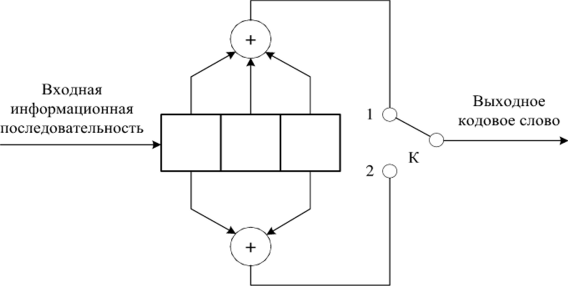
\includegraphics[scale=0.8]{coder}

  \begin{tabular}{ | c | c | c | c | c | c | c | c | c | c | }
    \hline
    Входной сигнал &1&0&1&1&1&1&0&0&1\\
    \hline
    Выходной сигнал &11&10&00&01&10&10&01&11&11\\
    \hline
  \end{tabular}
\end{center}

\begin{tikzpicture}[x=1.2cm, y=-1cm]
    \node at (-0.5,0) [left] {$s_1=00$};
    \node at (-0.5,1) [left] {$s_2=10$};
    \node at (-0.5,2) [left] {$s_3=01$};
    \node at (-0.5,3) [left] {$s_4=11$};

    % Nodes
    \foreach \x in {0,...,9} {
        \node at (\x,-.7) {$\x$};
        \foreach \y in {0,...,3} {
            \node (s\x\y) at (\x,\y) [circle,fill=blue] {};
        }
    }

    % Edges
    \trellisEdges{0}{0}
    \trellisEdges{1}{0}
    \trellisEdges{1}{1}
    \trellisEdges{2}{0}
    \trellisEdges{2}{1}
    \trellisEdges{2}{2}
    \trellisEdges{2}{3}
    \trellisEdges{3}{0}
    \trellisEdges{3}{1}
    \trellisEdges{3}{2}
    \trellisEdges{3}{3}
    \trellisEdges{4}{0}
    \trellisEdges{4}{1}
    \trellisEdges{4}{2}
    \trellisEdges{4}{3}
    \trellisEdges{5}{0}
    \trellisEdges{5}{1}
    \trellisEdges{5}{2}
    \trellisEdges{5}{3}
    \trellisEdges{6}{0}
    \trellisEdges{6}{1}
    \trellisEdges{6}{2}
    \trellisEdges{6}{3}
    \trellisEdges{7}{0}
    \trellisEdges{7}{1}
    \trellisEdges{7}{2}
    \trellisEdges{7}{3}
    \trellisEdges{8}{0}
    \trellisEdges{8}{1}
    \trellisEdges{8}{2}
    \trellisEdges{8}{3}

    % Inputs and Outputs
    \node at (-0,5) [left] {Входной бит};
    \node at (-0,6) [left] {Выходной бит};

    \trellisInOut{0}{0.5}{1}{11}
    \trellisInOut{1}{1.5}{0}{10}
    \trellisInOut{2}{1.5}{1}{00}
    \trellisInOut{3}{2}{1}{01}
    \trellisInOut{4}{3}{1}{10}
    \trellisInOut{5}{3}{1}{10}
    \trellisInOut{6}{2.5}{1}{01}
    \trellisInOut{7}{1}{0}{11}
    \trellisInOut{8}{0}{1}{11}
\end{tikzpicture}



\end{document}
